\section{Perspective}

\begin{frame}{\secname}{}
    We can use angles to represent the perspective of a point in the image if we know the focal distance $f$ of the camera.
    \begin{multicols}{2}
        \begin{figure}
        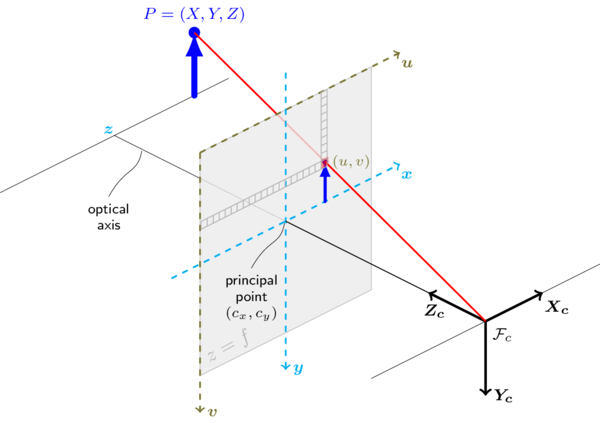
\includegraphics[width=0.6\textwidth]{img/fov.png}
    \end{figure}
    \phantom{}
    \vfill
    \begin{gather*}
        \alpha = \arctan\frac{u}{f}
    \end{gather*}
    \vfill
    \phantom{}
    \end{multicols}
\end{frame}

\begin{frame}{\secname}{Use case: Locate the place from where a photo was taken}
    We can use this information to locate where a photo was taken.
    \begin{figure}
        \centering
        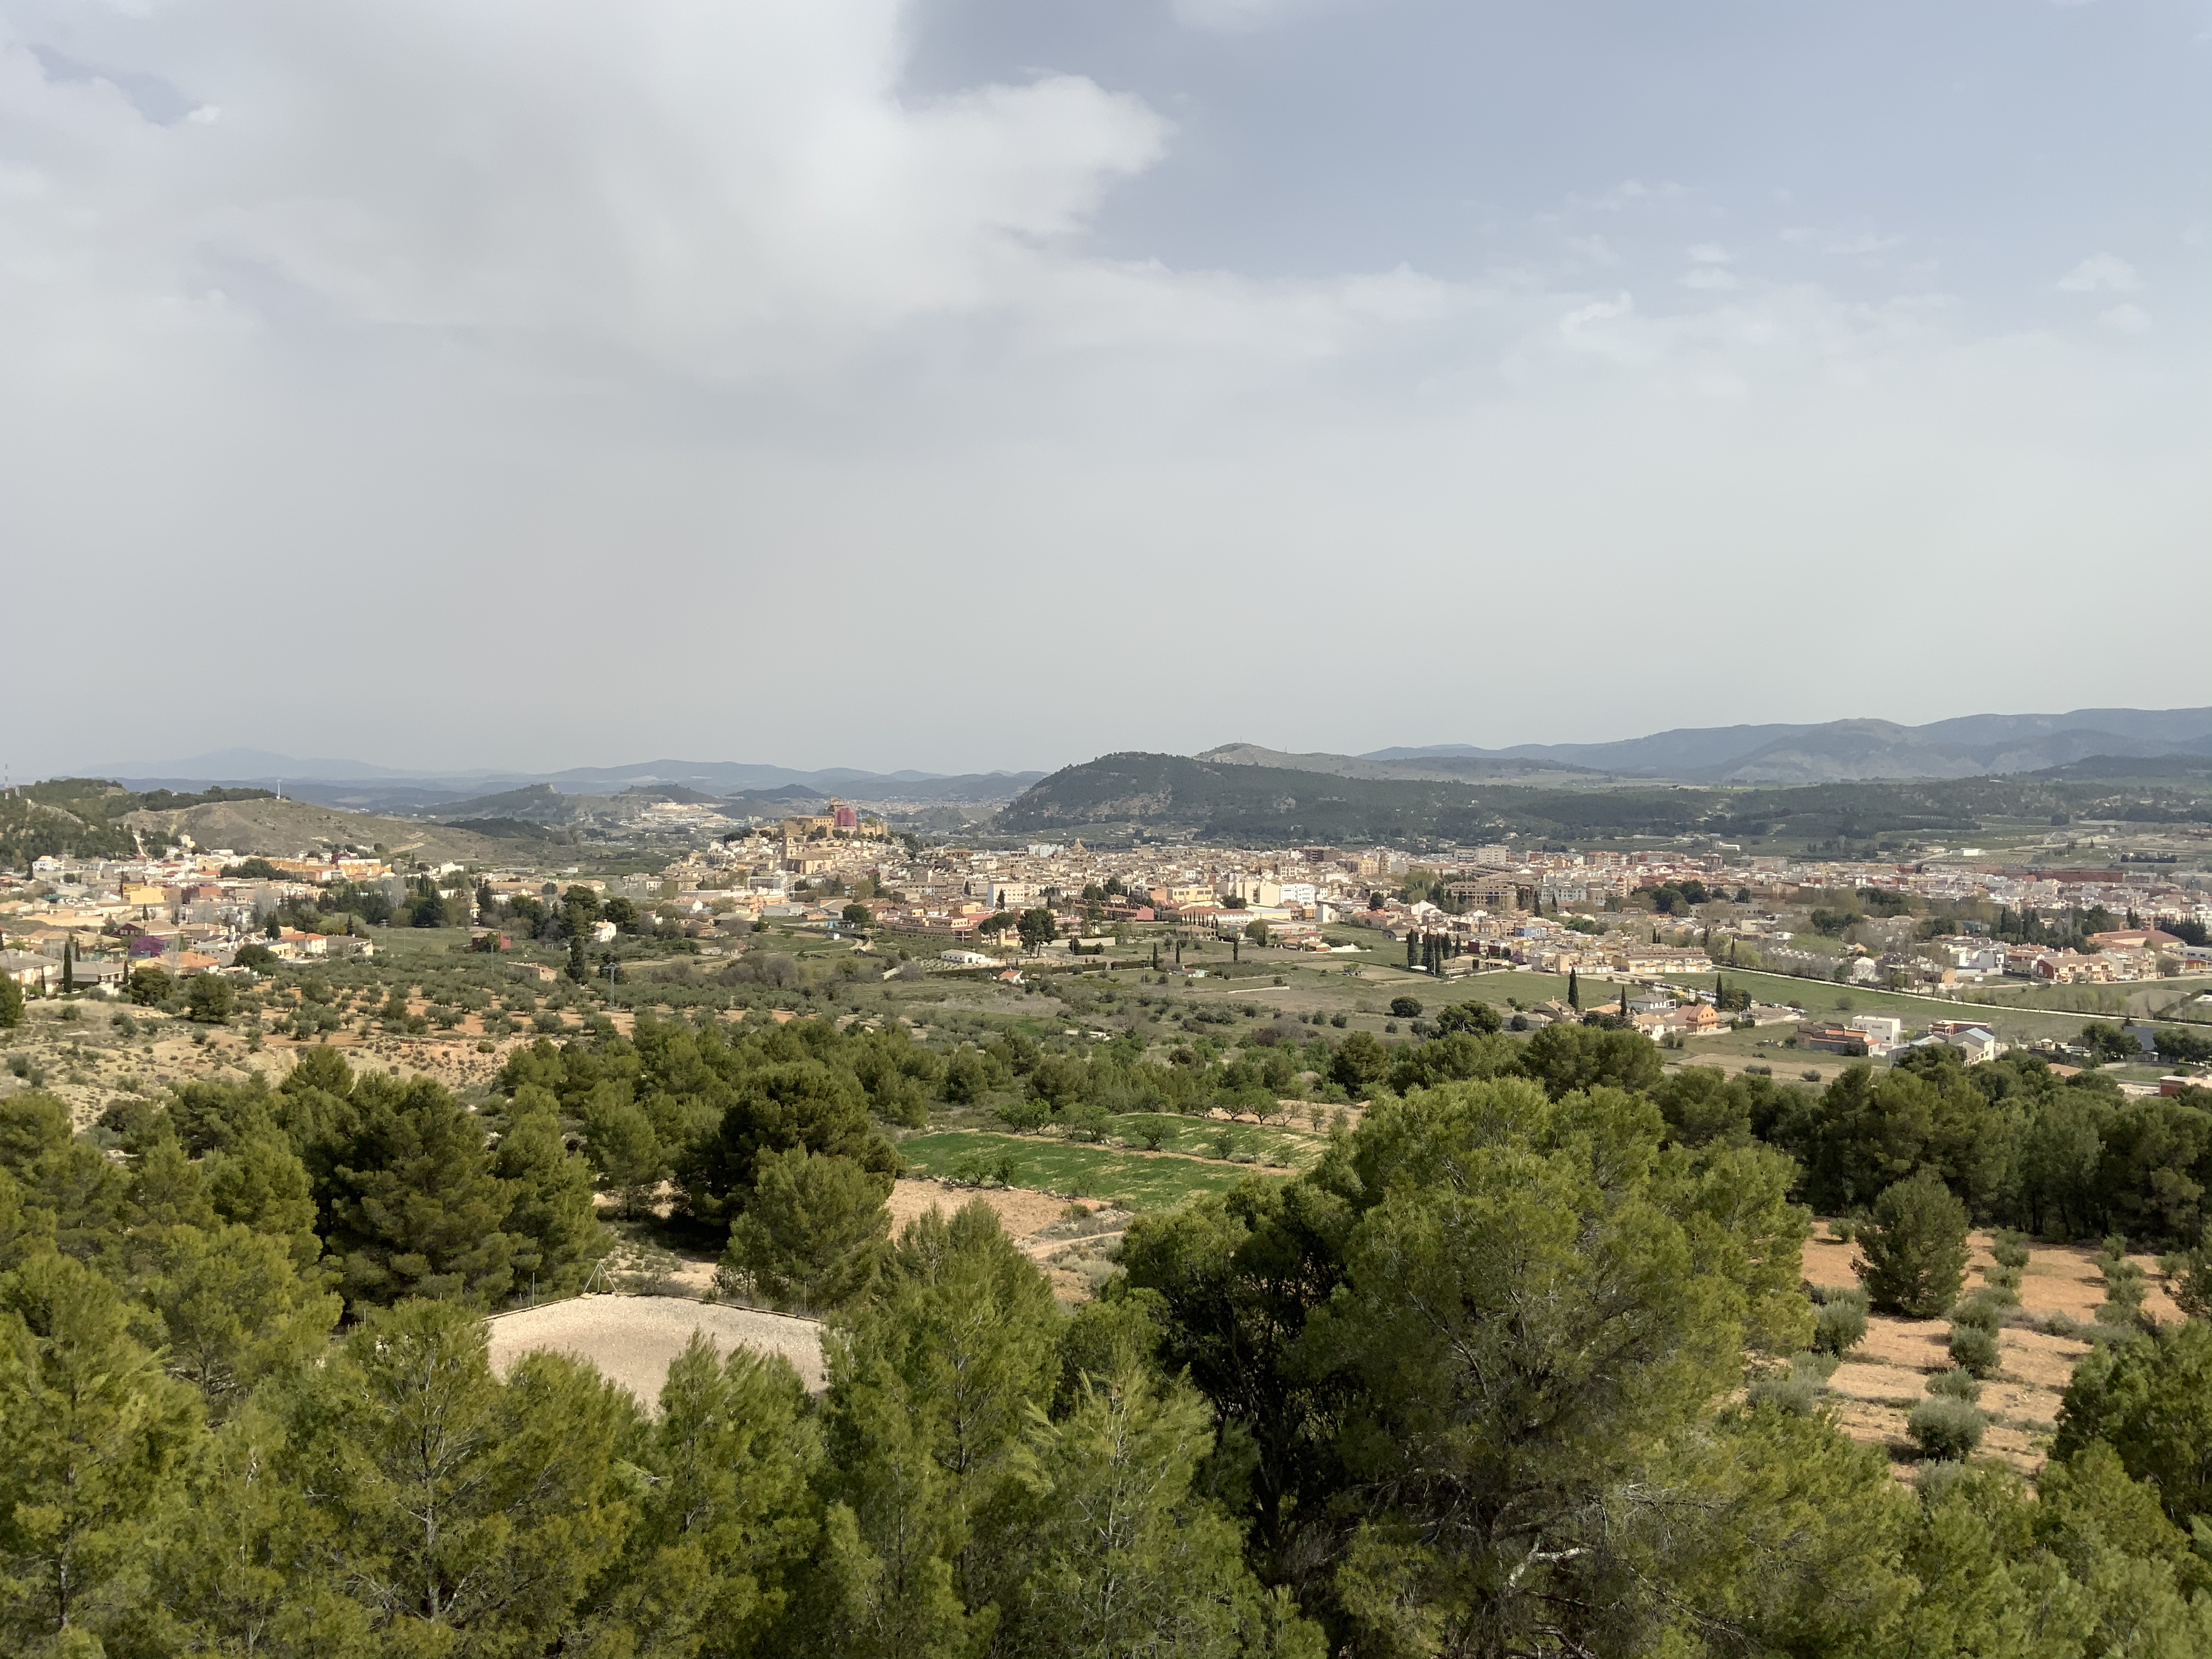
\includegraphics[width=0.6\textwidth]{img/mirador1_ipad.jpeg}
    \end{figure}
\end{frame}

\begin{frame}{\secname}{Use case: Locate the place from where a photo was taken}
    We only need to use some trigonometry.
    \begin{figure}
        \subfloat{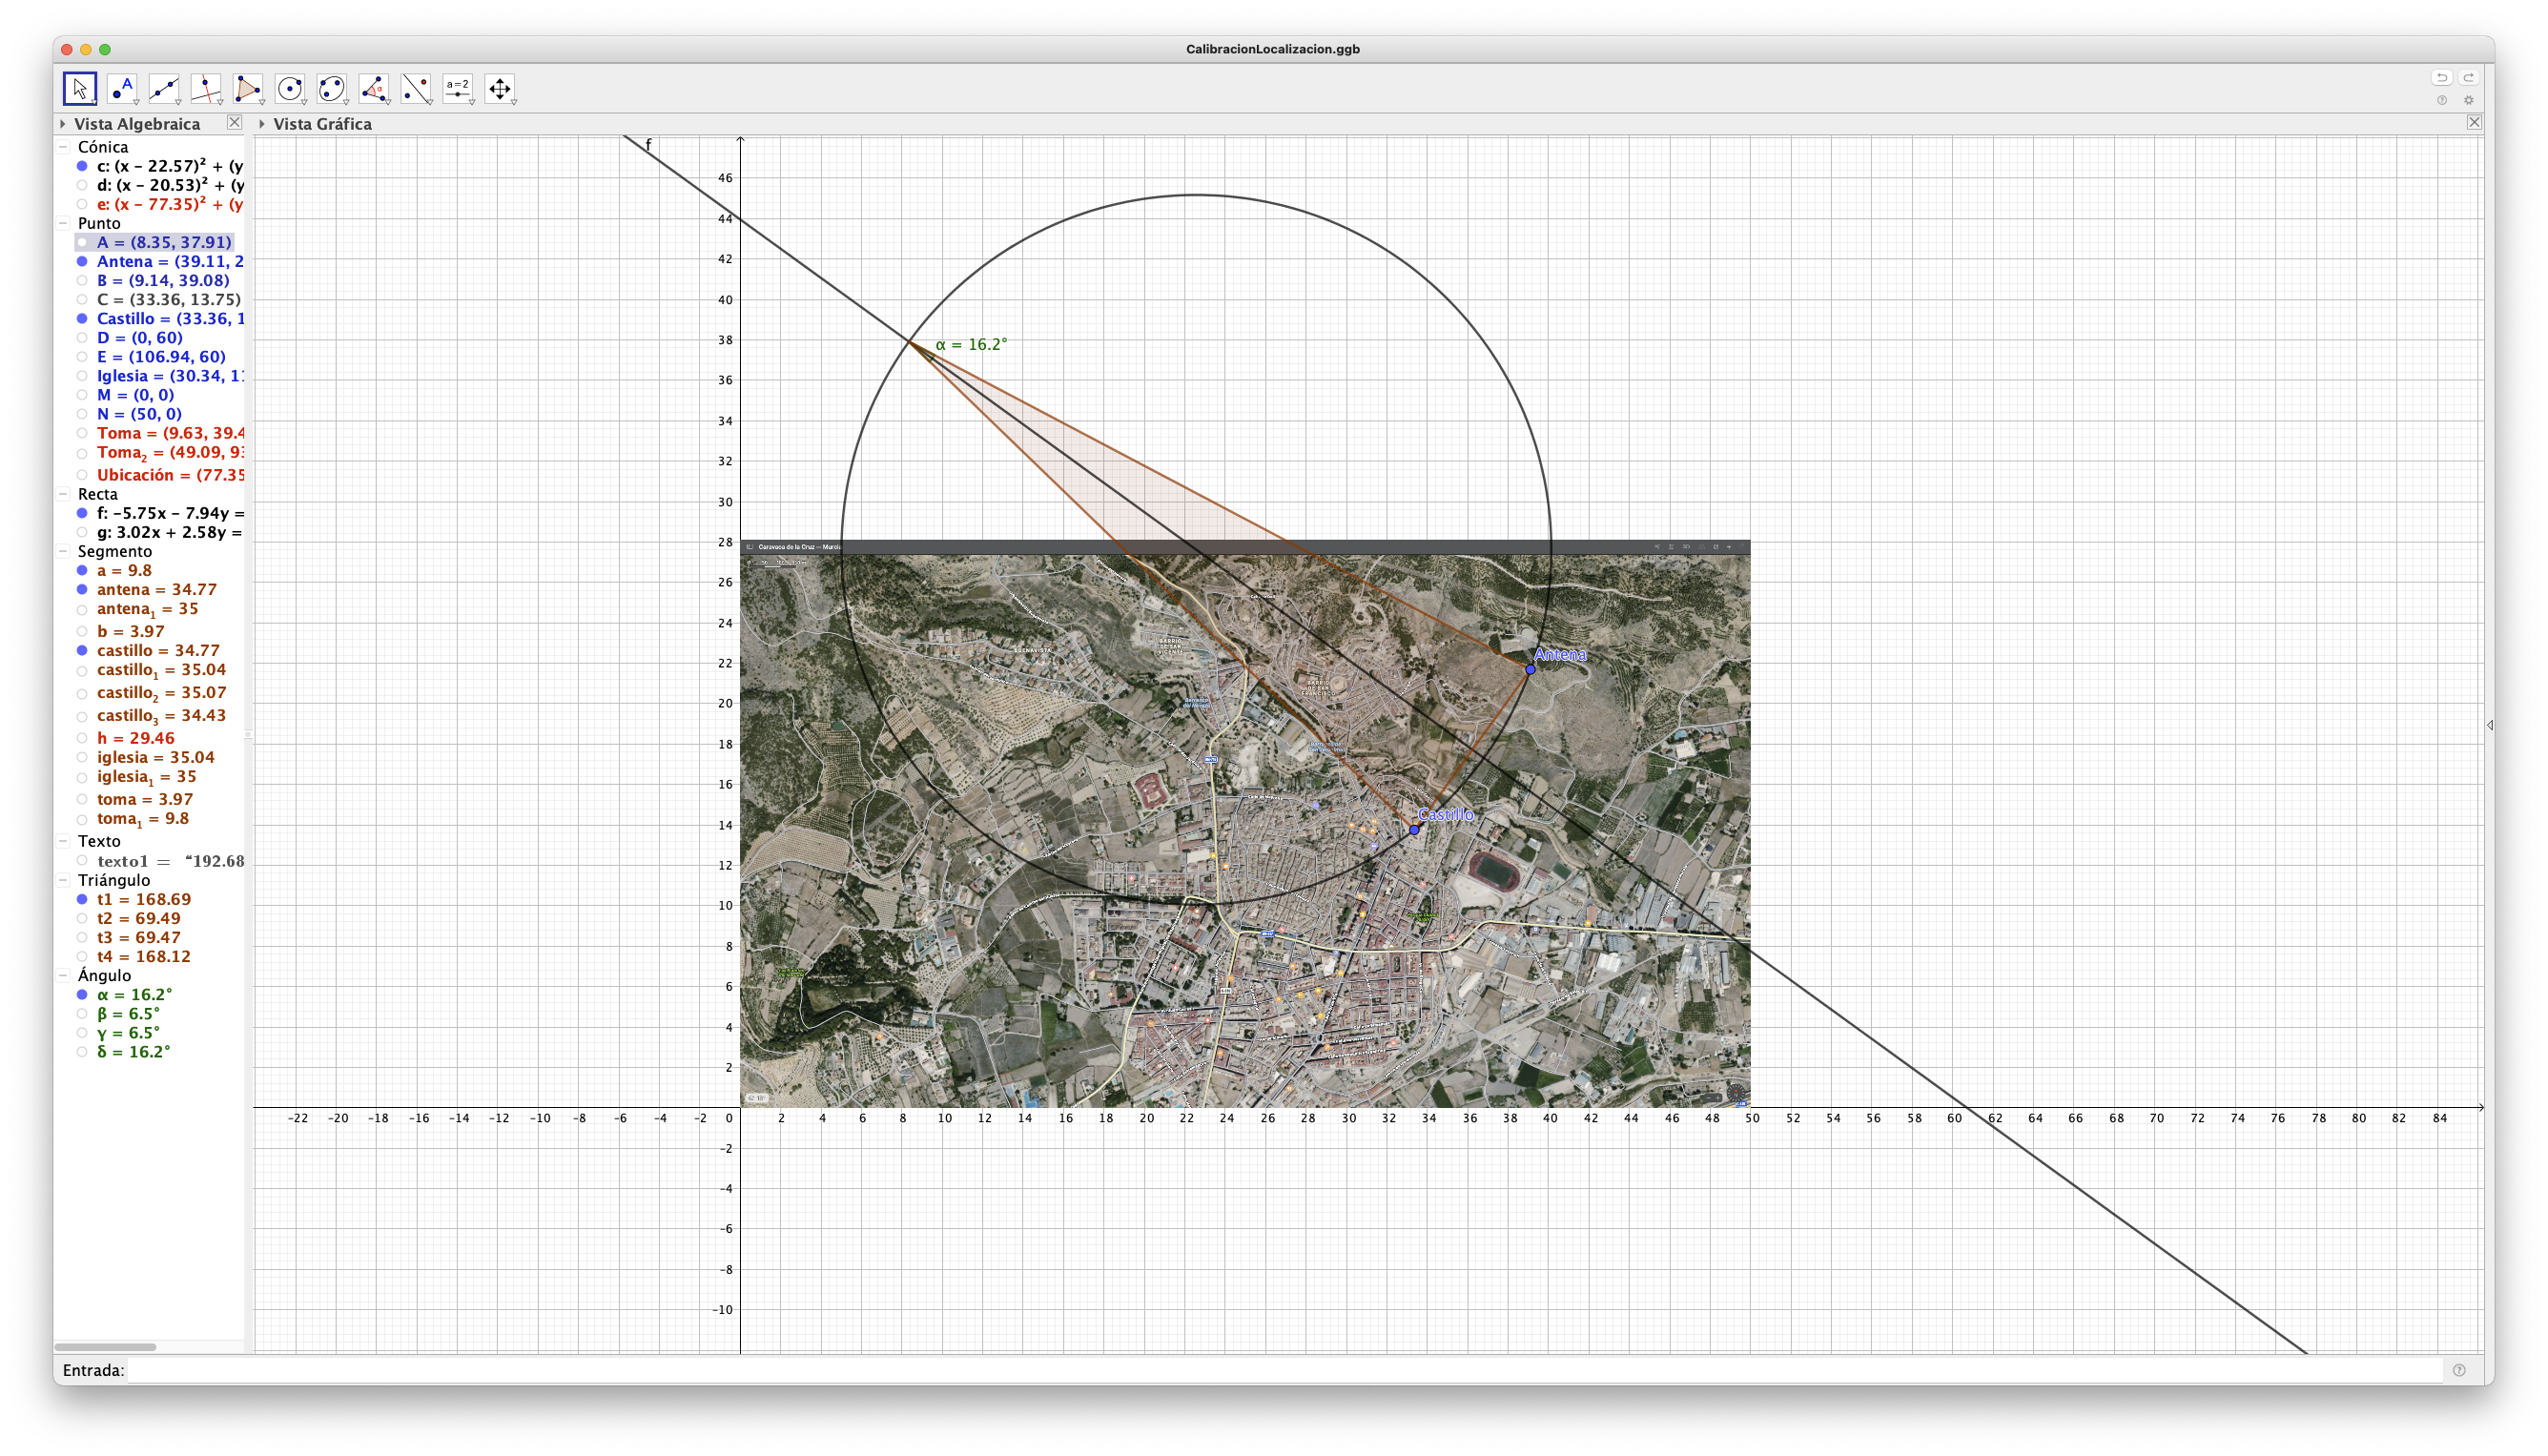
\includegraphics[width=0.5\textwidth]{img/Circ-Antena-Castillo.png}}
        \subfloat{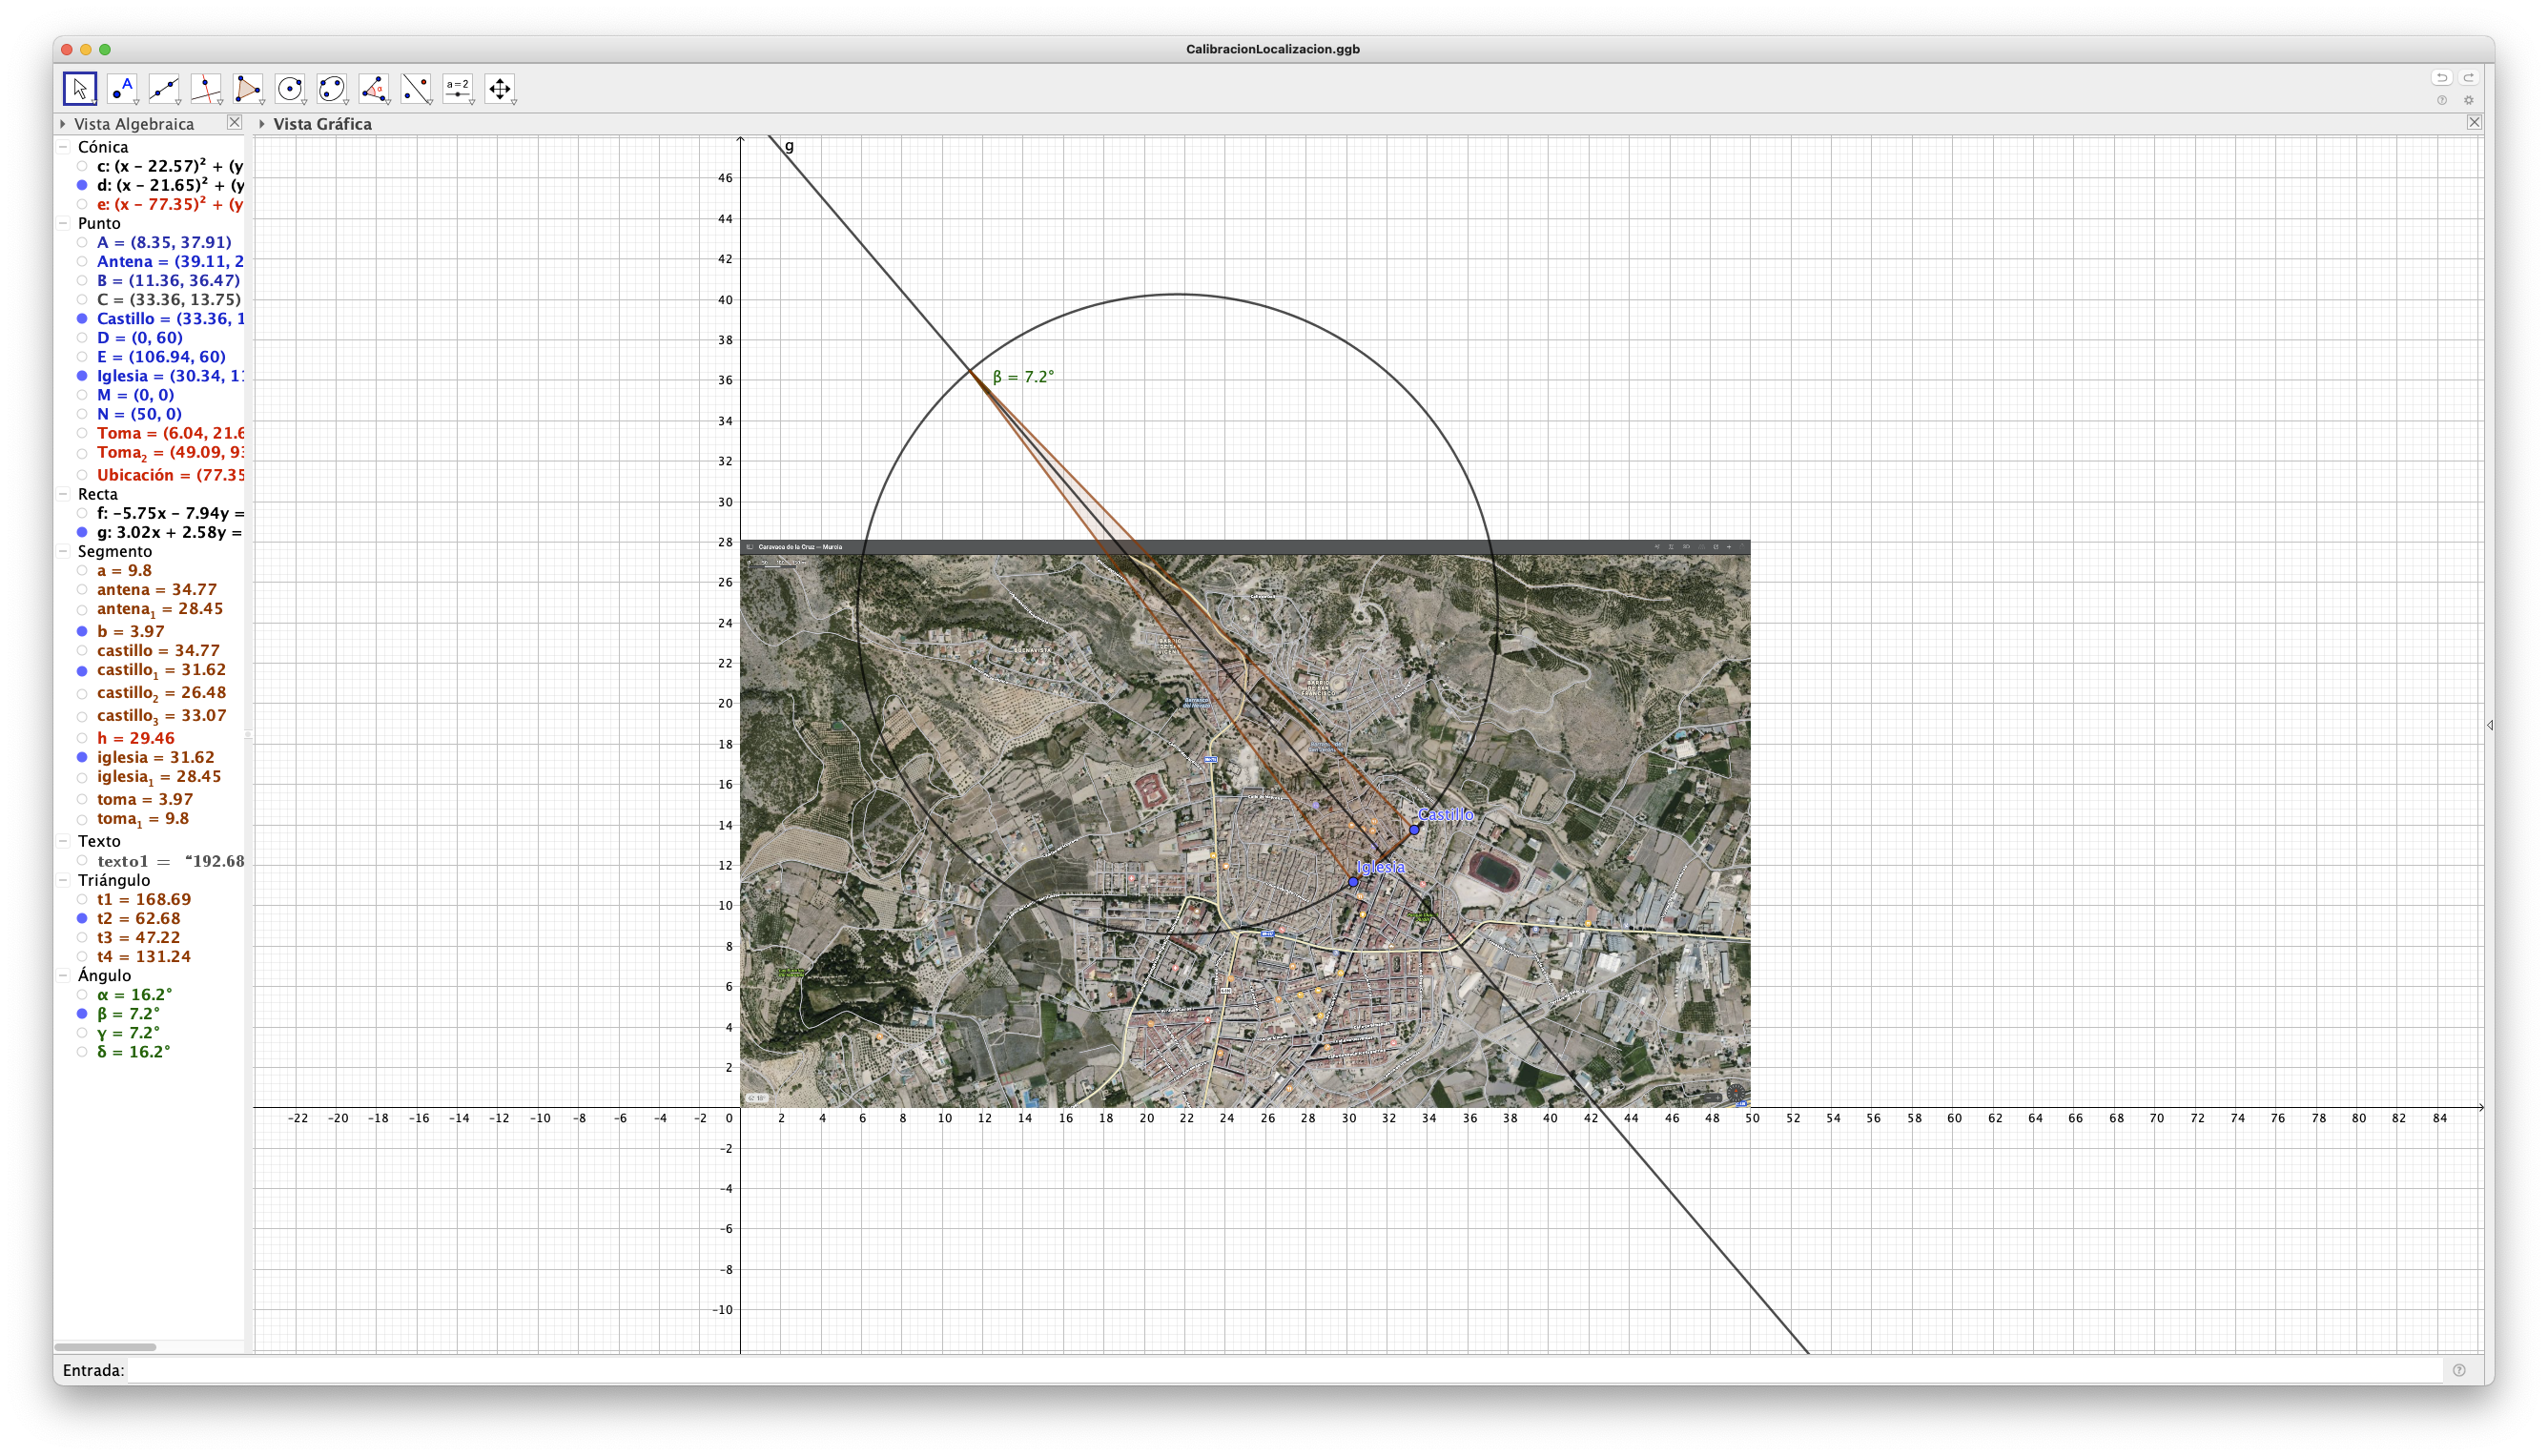
\includegraphics[width=0.5\textwidth]{img/Circ-Castillo-Iglesia.png}}
    \end{figure}    
\end{frame}

\begin{frame}{\secname}{Use case: Locate the place from where a photo was taken}
    \begin{figure}
        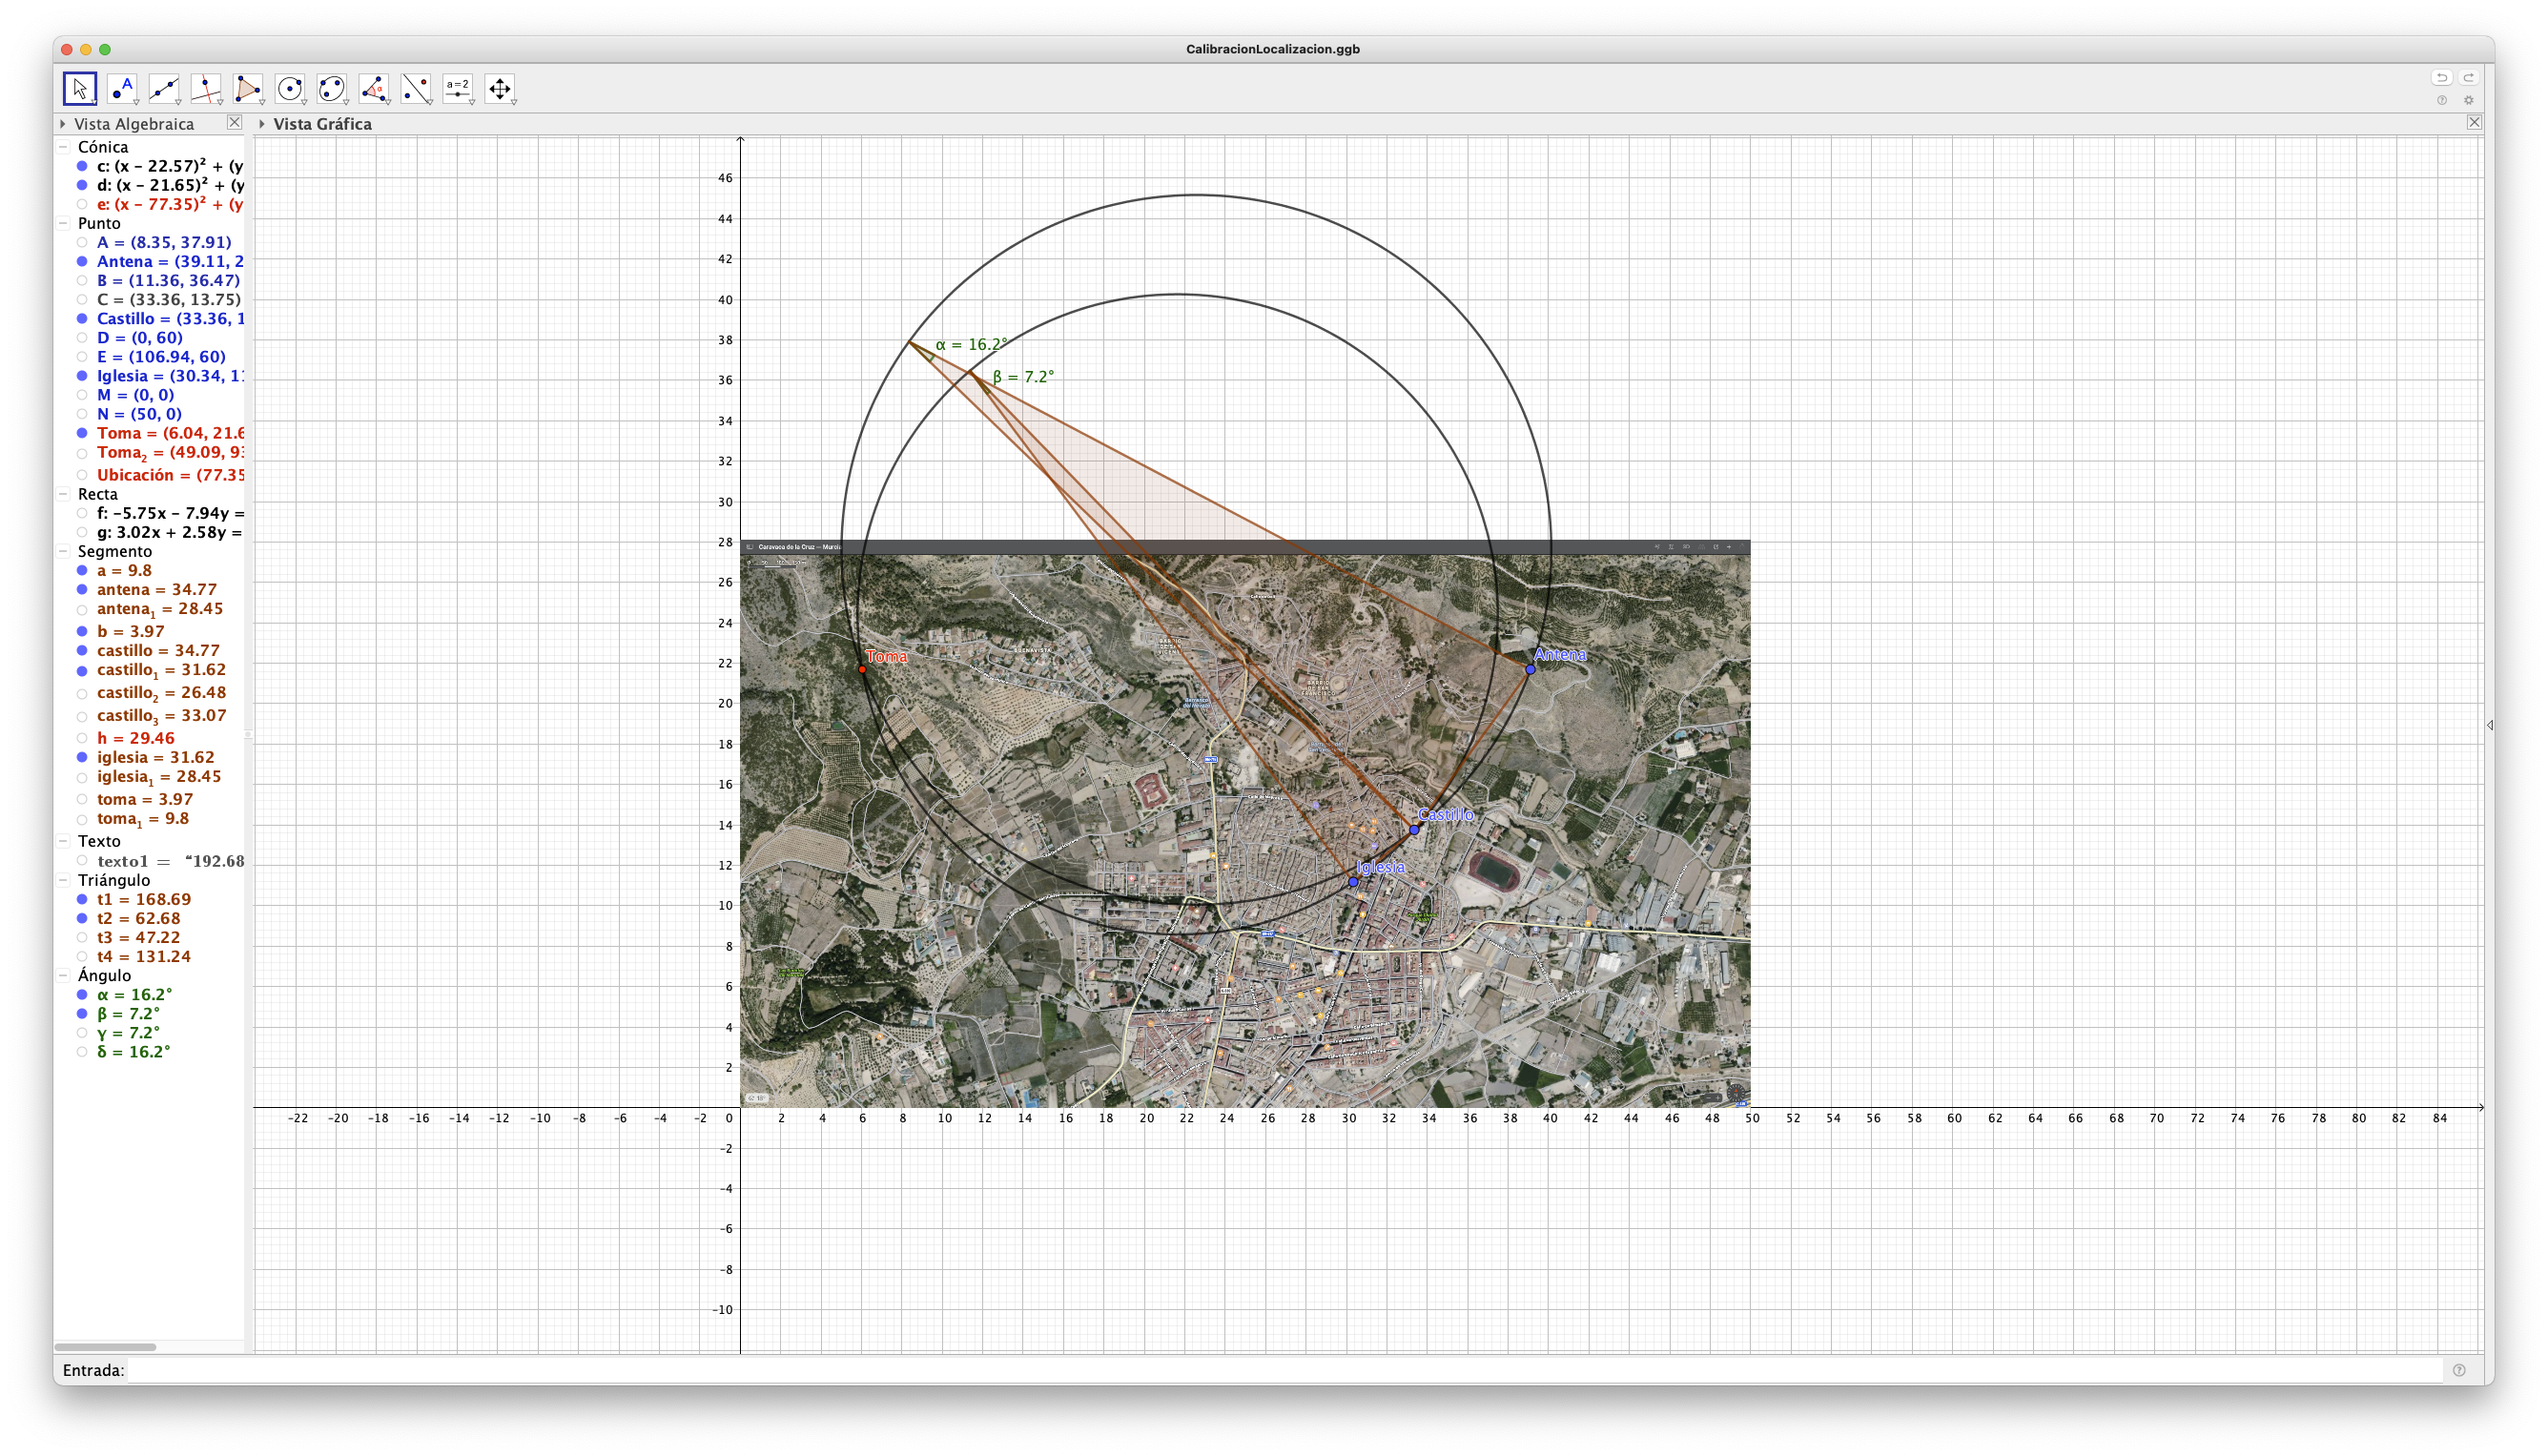
\includegraphics[width=0.9\textwidth]{img/Inter-Circs.png}
    \end{figure}
\end{frame}

\begin{frame}{Perspective}{Use case: Locate the place from where a photo was taken}
    The precision is quite accurate even though the methods are not so precise.
    \begin{figure}
        \subfloat{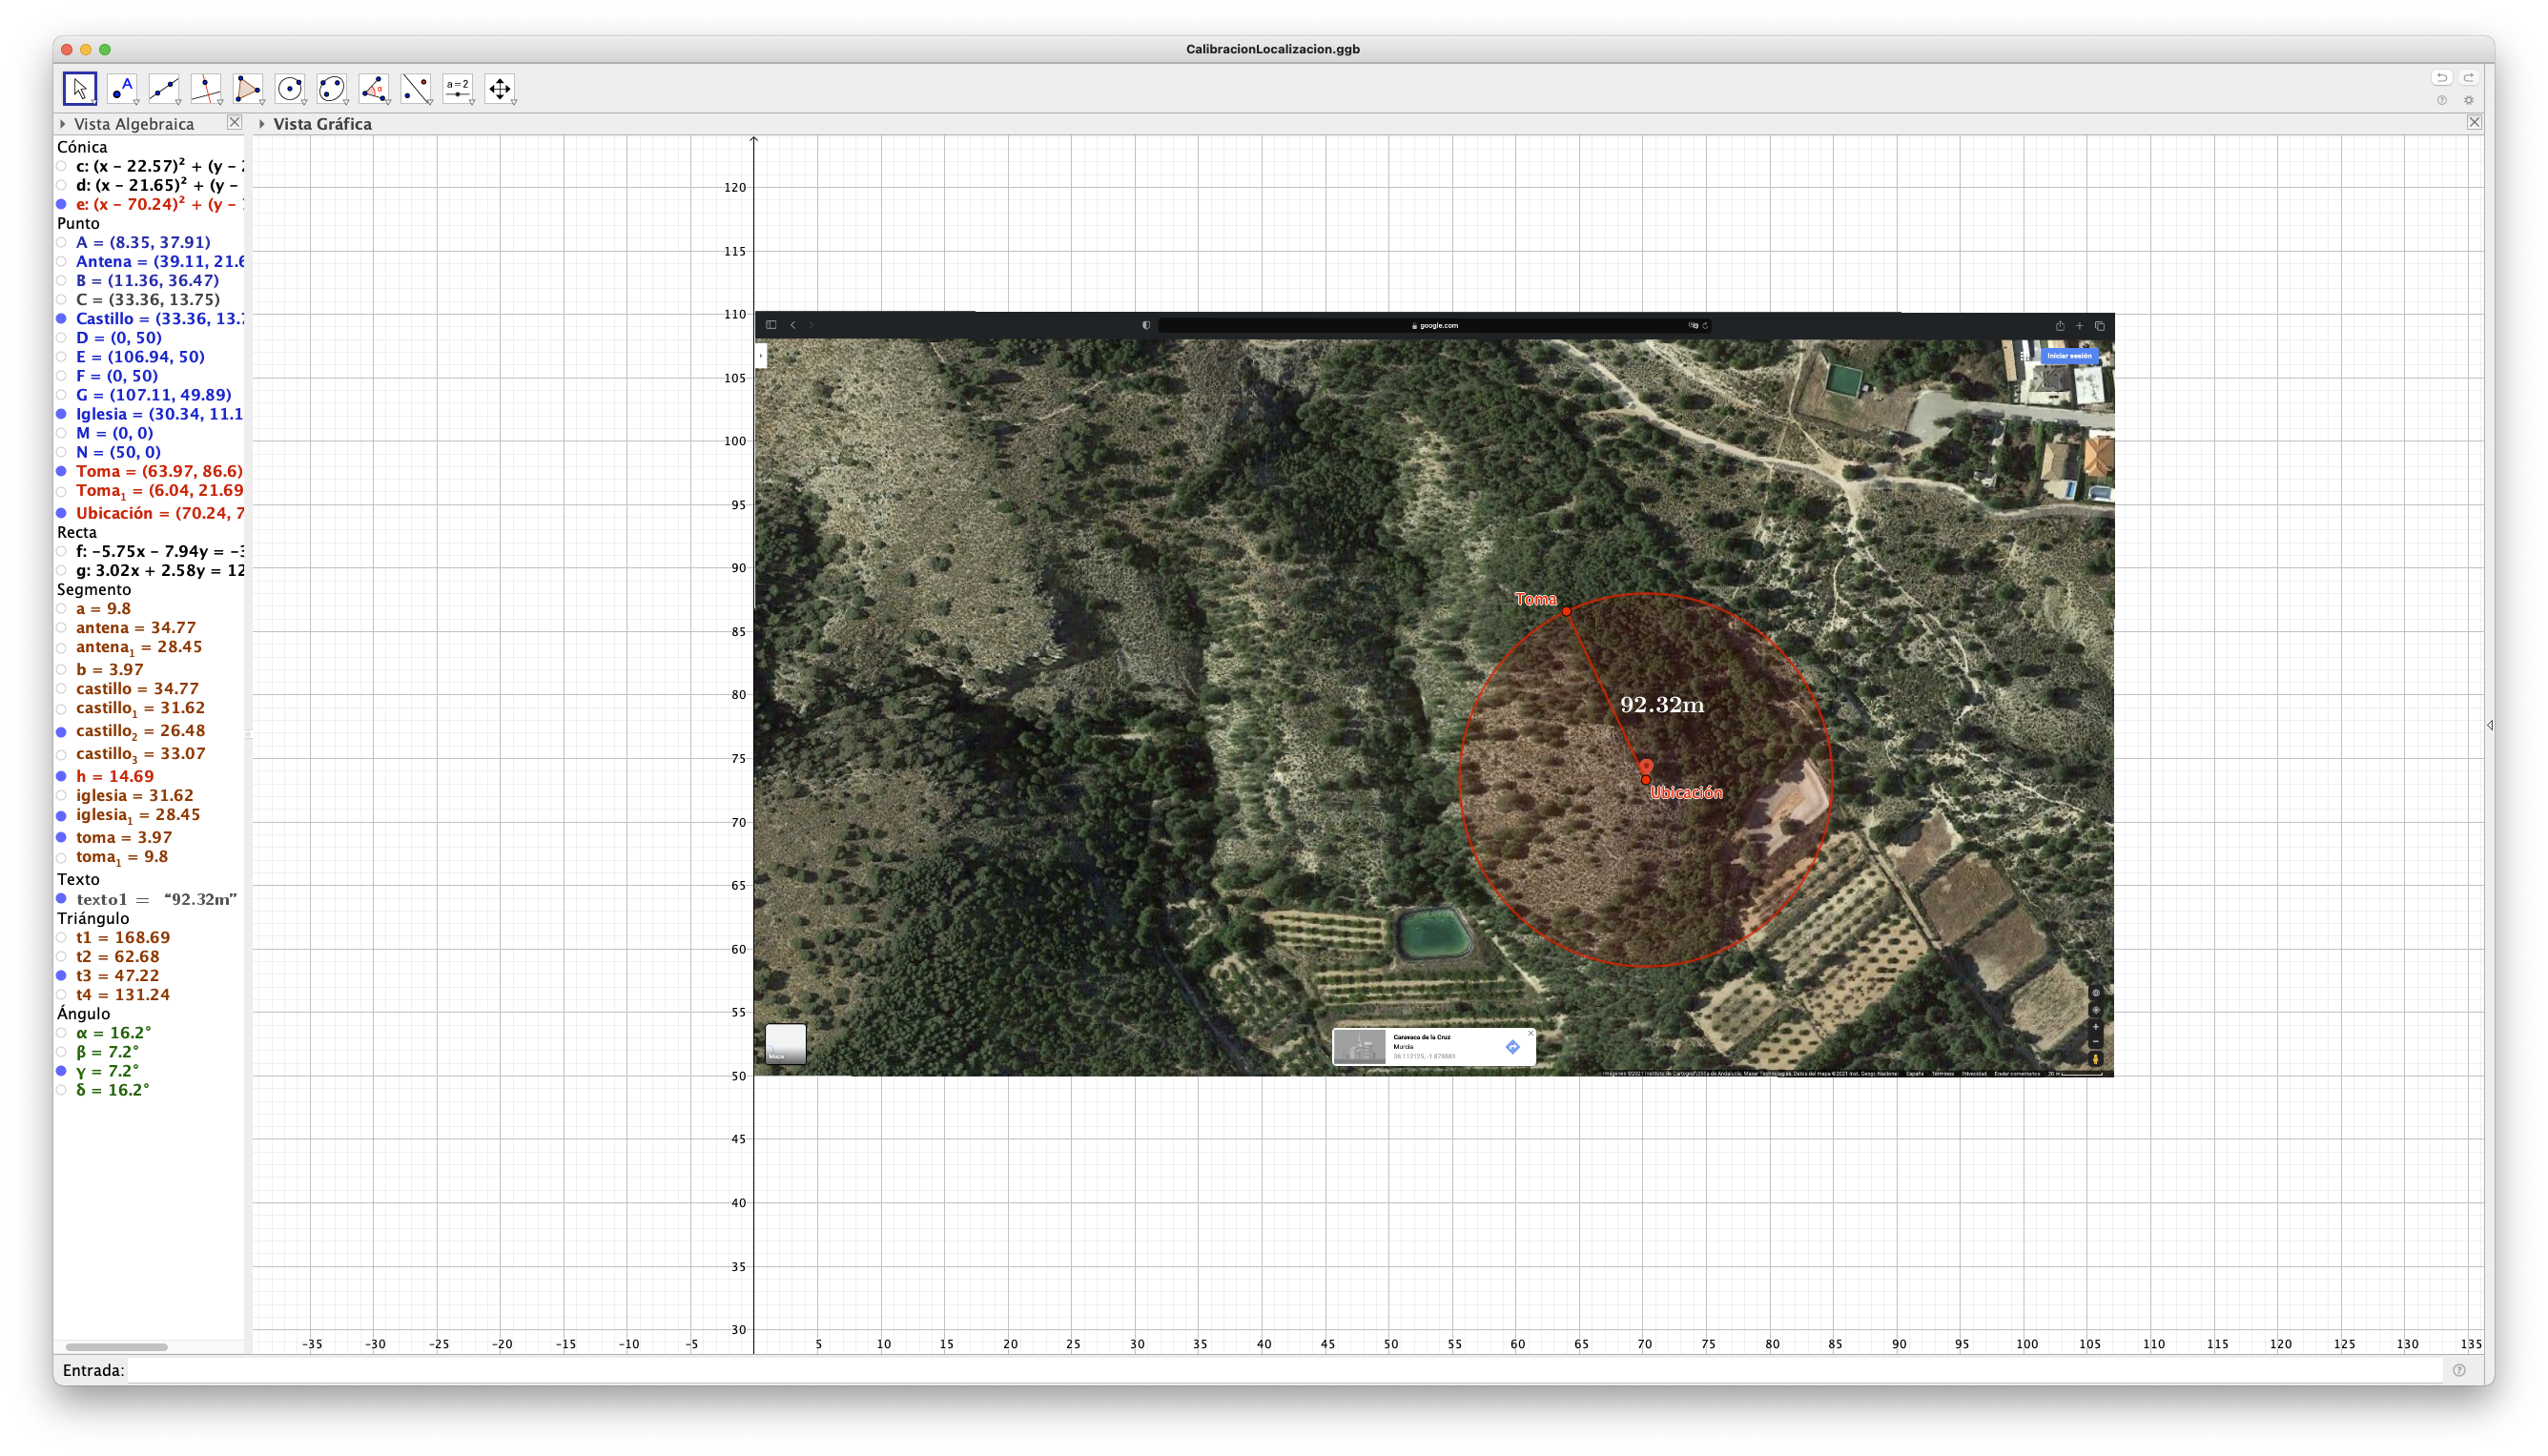
\includegraphics[width=0.9\textwidth]{img/error-medida.png}}
    \end{figure}
\end{frame}

